% !TEX root = thesis.tex

%%
%%
%% further research
%%
%%


%%%%%%%%%%%%%%%%%%%%%%%%%%%%%%%%%%%%%%%%%%%%%%%%%%%%%%%%%%%%%%%%%%%%%%%%%%%%%%
%%
%% Section: Distance between the population and risk function peaks
%%
%%%%%%%%%%%%%%%%%%%%%%%%%%%%%%%%%%%%%%%%%%%%%%%%%%%%%%%%%%%%%%%%%%%%%%%%%%%%%%
\section{Distance between the population and risk function peaks}
\label{sec:results:p1.4_Gap_risk}

%%%%%%%%%%%%%%%%%%%%%%%%%%%%%
% Parameter table
%%%%%%%%%%%%%%%%%%%%%%%%%%%%%
\begin{table}[htbp]
    \centering
    \begin{tabular}{ll}
        \toprule
        Parameter & Value \\
        \midrule
        Population size & 10,000 \\
        Population \gls{spread} & 1.4 \\
        Population center & (-0.5,0), (-1,0), (-1.5,0), (-2,0) \\
        \Gls{factor} & 40, 60 \\
        Incident \gls{spread} & 1.0 \\
        Incident center & (0.5,0), (1,0), (1.5,0), (2,0) \\
        \bottomrule
    \end{tabular}
    \caption{Parameters used for varying the peak of the single-peak risk function with \glspl{factor} 100 and the peak of the single-peak population of 10,000}
    \label{tab:params:p1.4_100_Gap_risk}
\end{table}

In this section, we look at incident risk function that have their peak at a different location from the peak in the population distribution.
We expect that as this distance grows, the relatively small population at the peak of the incident risk will make it difficult to obtain any information through observing incidents and estimating with the \gls{dkd}.
The results of the experiments described in this section are summarized in \Cref{tab:mean_error_rates:p1.4_100_1_1h_1s,tab:mean_error_rates:p1.4_100_1_1h_2s,tab:mean_error_rates:p1.4_100_1_1h_3s,tab:mean_error_rates:p1.4_100_1_1h_4s}.

%%%%%%%%%%%%%%%%%%%%%%%%%%%%%%%%%%%%%%%%%%%%%%%%%
% Examples showing distance between population
% and incident peaks
%%%%%%%%%%%%%%%%%%%%%%%%%%%%%%%%%%%%%%%%%%%%%%%%%
\begin{figure}[htbp]
    \centering
    \begin{subfigure}{0.45\textwidth}
        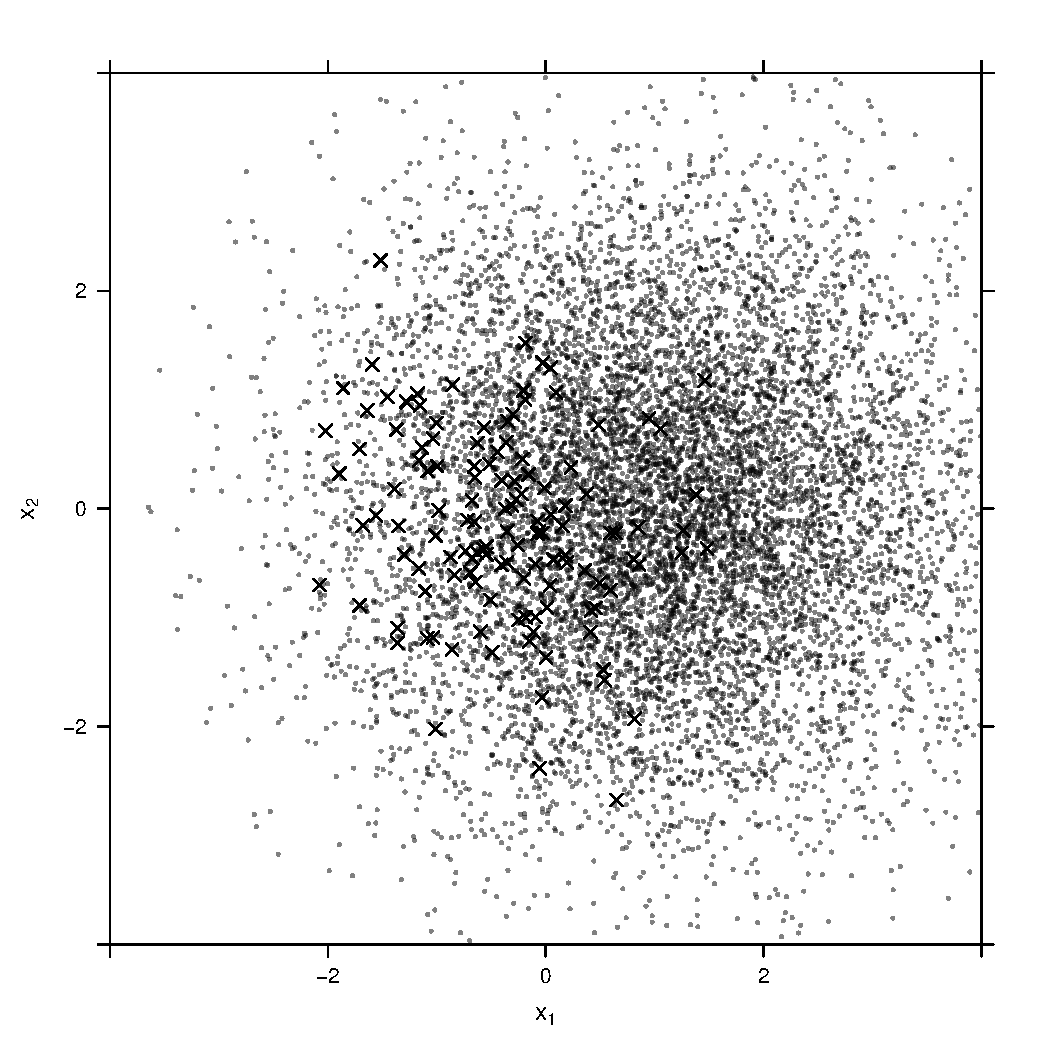
\includegraphics[width=\textwidth]{results/p1.4_100_1_1h_2s/output/population_and_incidents_scatter}
        \subcaption{Centers at $\{(-1,0), (1,0)\}$ (distance 2)}
        \label{fig:one_sample:p1.4_100_Gap_risk:2}
    \end{subfigure}
    \begin{subfigure}{0.45\textwidth}
        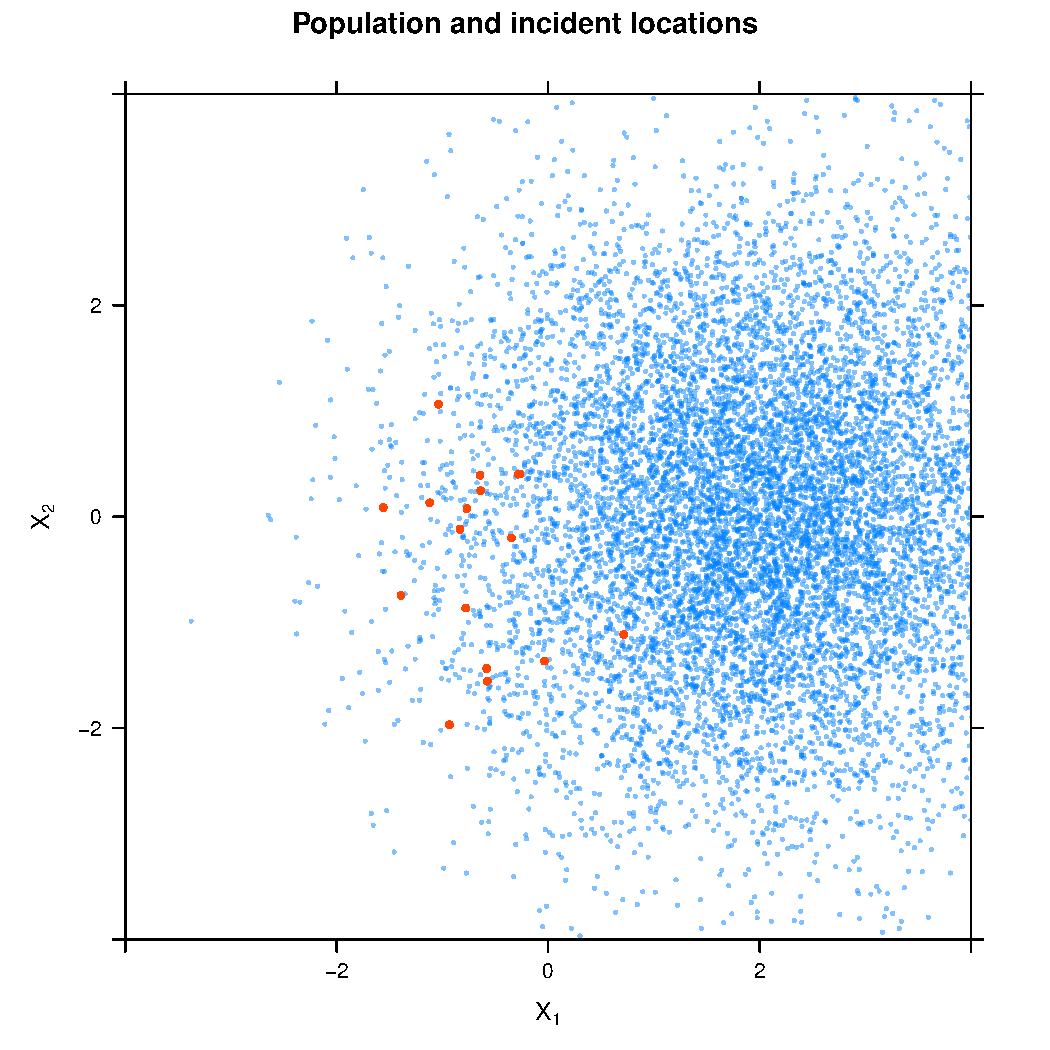
\includegraphics[width=\textwidth]{results/p1.4_100_1_1h_4s/output/population_and_incidents_scatter}
        \subcaption{Centers at $\{(-2,0), (2,0)\}$ (distance 4)}
        \label{fig:one_sample:p1.4_100_Gap_risk:4}
    \end{subfigure}
    \caption[Examples showing distance between population and incident peaks]
        {A single realization of different sample sizes from a single-peak risk on a single-peak population, obtained by varying the distance between two peaks. \scatterplotcaption.}
    \label{fig:one_sample:p1.4_100_Gap_risk}
\end{figure}

%%%%%%%%%%%%%%%%%%%%%%%%%%%%%%%%%%%%%%%%%%%%%%%%%
% MISE by distance between population
% and incident peaks
%%%%%%%%%%%%%%%%%%%%%%%%%%%%%%%%%%%%%%%%%%%%%%%%%
\begin{figure}[htbp]
    \centering
    \begin{subfigure}[b]{0.49\textwidth}
        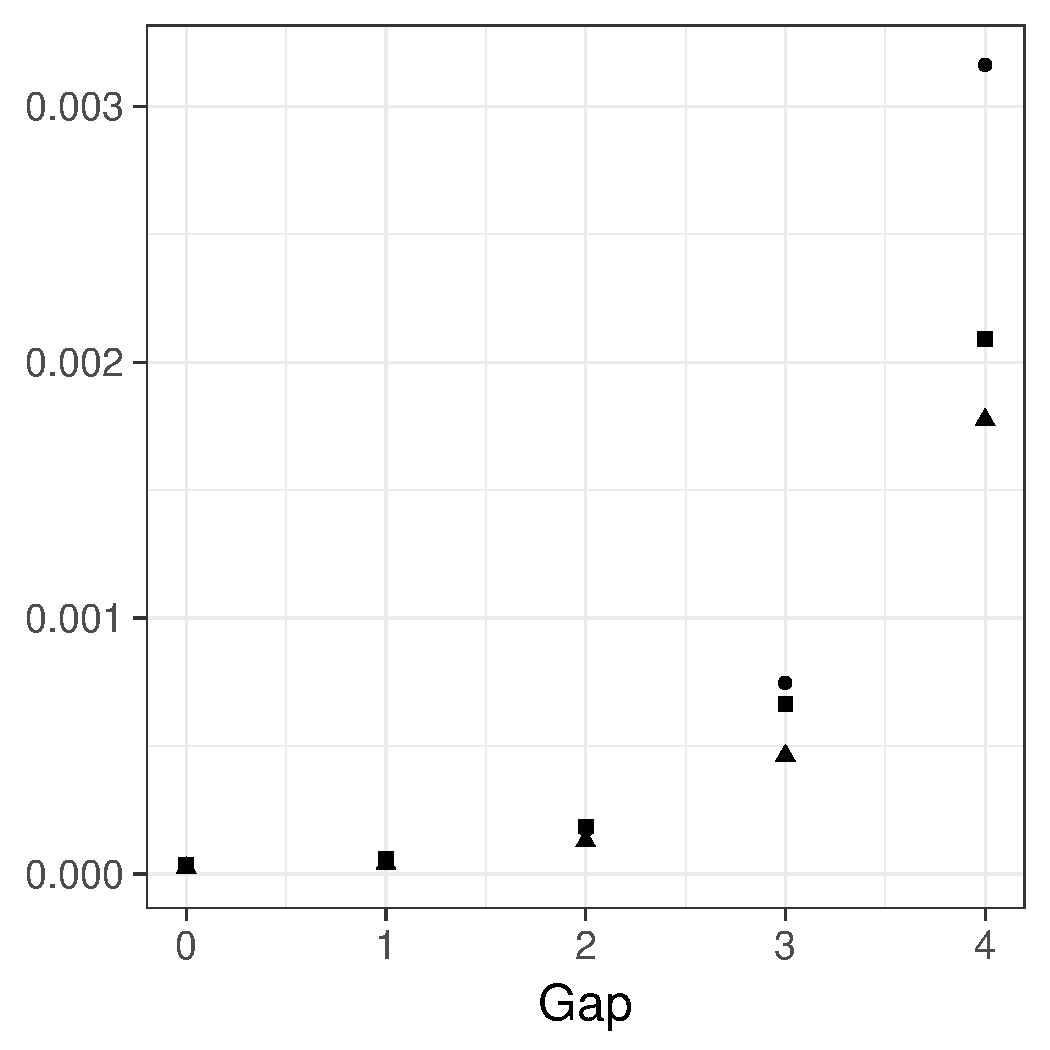
\includegraphics[width=\textwidth]{results/by_pop_risk_distance/MISE-vs-population-risk-gap}
        \caption{\glsentryname{mise}}
        \label{fig:ise:p1.4_100_Gap_risk:mise}
    \end{subfigure}
    \begin{subfigure}[b]{0.49\textwidth}
        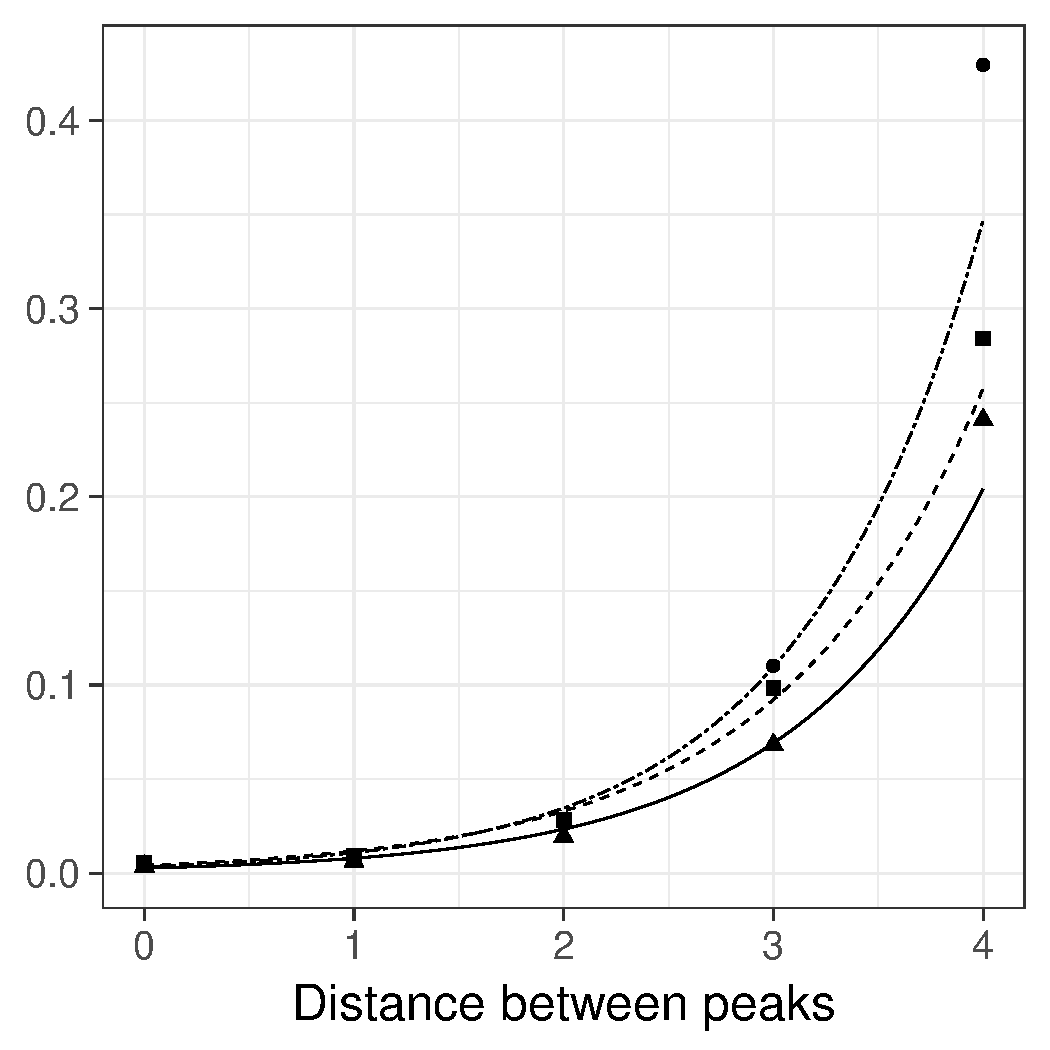
\includegraphics[width=\textwidth]{results/by_pop_risk_distance/RMISE-vs-population-risk-gap}
        \caption{\glsentryname{rmise}}
        \label{fig:ise:p1.4_100_Gap_risk:rmise}
    \end{subfigure}

    \begin{subfigure}[b]{0.49\textwidth}
        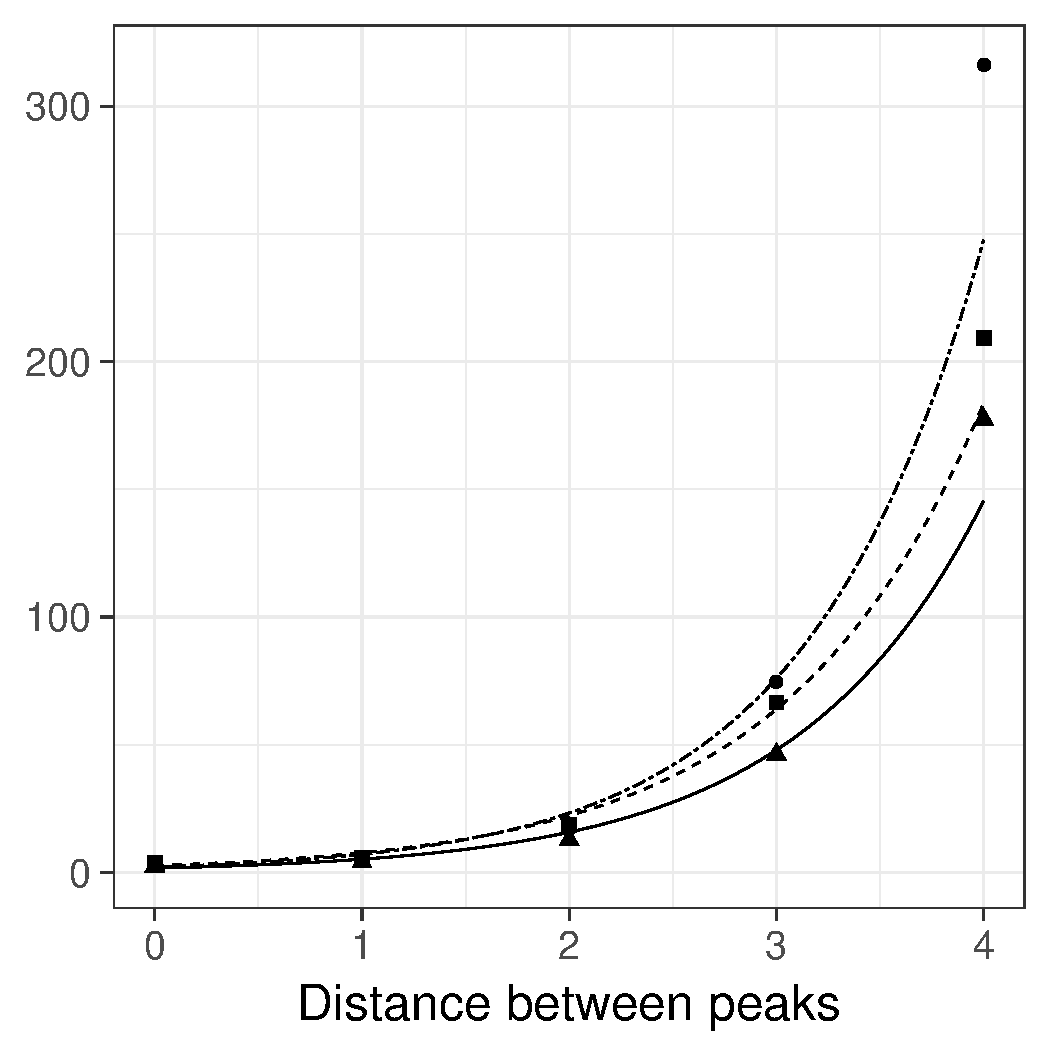
\includegraphics[width=\textwidth]{results/by_pop_risk_distance/NMISE-vs-population-risk-gap}
        \caption{\glsentryname{nmise}}
        \label{fig:ise:p1.4_100_Gap_risk:nmise}
    \end{subfigure}
    \begin{subfigure}[b]{0.49\textwidth}
        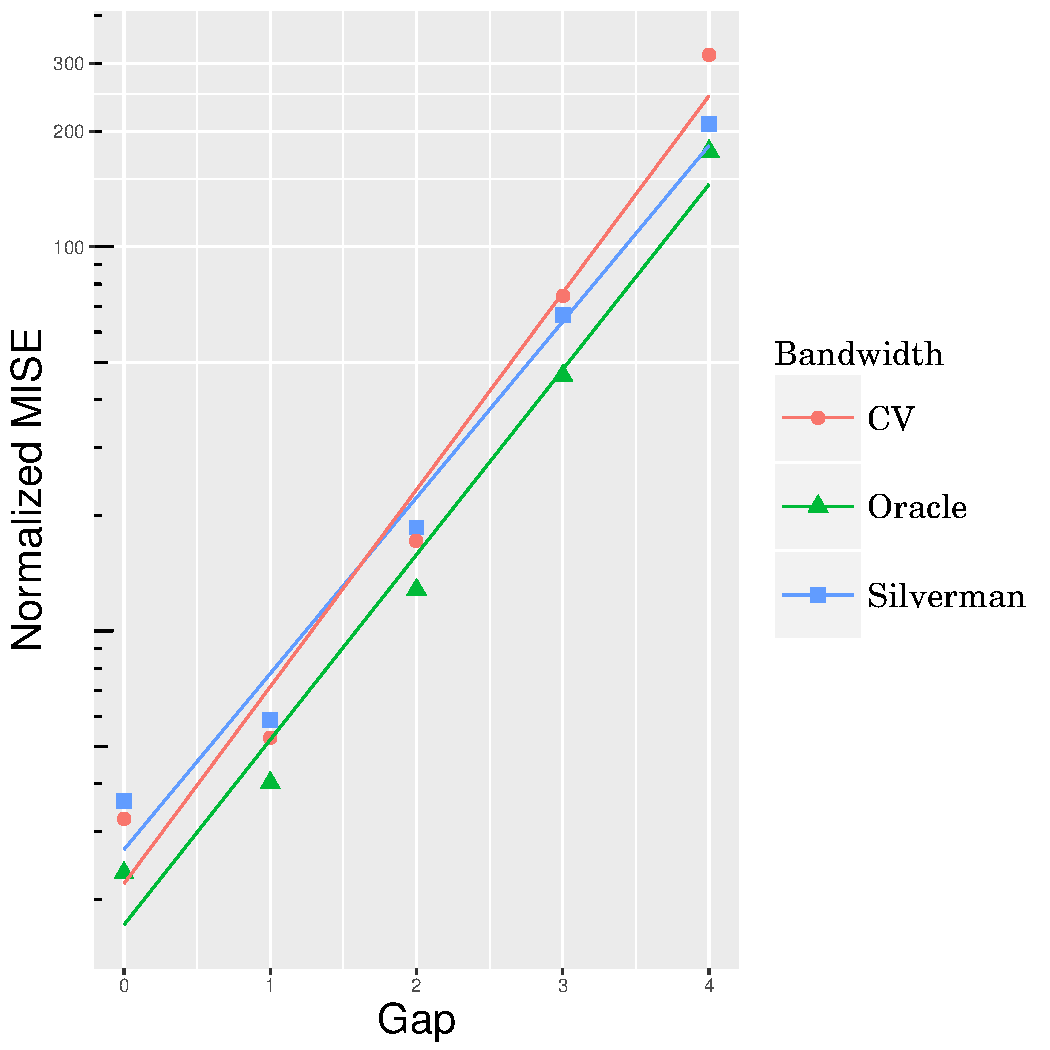
\includegraphics[width=\textwidth]{results/by_pop_risk_distance/NMISE-vs-population-risk-gap-log-log}
        \caption{Log-log of \glsentryname{nmise}}
        \label{fig:ise:p1.4_100_Gap_risk:nmise_log_log}
    \end{subfigure}    
    \caption[\glsentryname{mise} by distance between two risk peaks]
        {\glsentryname{mise} by distance between two risk peaks. \errorplotcaption}
    \label{fig:ise:p1.4_100_Gap_risk}
\end{figure}

%latex.default(df.alpha, title = "nmise_convergence_table", where = "htbp",     label = "tab:results:nmise_convergence_by_pop_incident_gap",     rowname = NULL, booktabs = TRUE, cdec = c(0, 3), caption.loc = "bottom",     caption = "NMISE convergence rate by incident-population peak distance for different bandwidth selectors for a single-peak risk function with spread of 1.0 on a single-peak population of 10,000.",     caption.lot = "NMISE Convergence rate by incident-population peak distance")%
\begin{table}[htbp]
\begin{center}
\begin{tabular}{lr}
\toprule
\multicolumn{1}{c}{Selector}&\multicolumn{1}{c}{Gap}\tabularnewline
\midrule
Oracle&$1.110$\tabularnewline
Silverman&$1.055$\tabularnewline
CV&$1.181$\tabularnewline
\bottomrule
\end{tabular}
\caption[NMISE Convergence rate by incident-population peak distance]{NMISE convergence rate by incident-population peak distance for different bandwidth selectors for a single-peak risk function with spread of 1.0 on a single-peak population of 10,000.\label{tab:results:nmise_convergence_by_pop_incident_gap}}\end{center}
\end{table}


\Cref{fig:ise:p1.4_100_Gap_risk} shows the different measures of \gls{mise} accuracy.
We can see from \Cref{fig:ise:p1.4_100_Gap_risk:nmise_log_log} that there is a linear relationship in the log-log graph,
indicating polynomial increase with positive coefficient of \gls{mise} when the distance between the incident and population peaks increases.
We see in \Cref{tab:results:nmise_convergence_by_pop_incident_gap} that the exponent is just over 1,
indicating just worse than linear.
